\documentclass[cjk,slidestop,compress,mathserif,blue]{beamer}
%dvipdfm选项是关键,否则编译统统通不过
%beamer的颜色选项定义的是导航条和标题的颜色(即关键词structure的颜色)

%%%%%%%%%%%%%%%%仅限于XeTeX可使用的宏包%%%%%%%%%%%%%%%%%%%%%%%%%%%%
\usepackage{fontspec,xunicode,xltxtra,beamerthemesplit}
%\usepackage{beamerthemesplit}
\usepackage{xeCJK}
\setCJKmainfont[BoldFont=黑体, ItalicFont=楷体, BoldItalicFont=仿宋]{黑体}
%\setsansfont[Mapping=tex-text]{Adobe 黑体 Std}
%如果装了Adobe Acrobat,可在font.conf中配置Adobe字体的路径以使用其中文字体
%也可直接使用系统中的中文字体如SimSun,SimHei,微软雅黑 等
%原来beamer用的字体是sans family;注意Mapping的大小写,不能写错

%%%%%%%%   确定标题和导航条结构的框架     %%%%%%%%%%%%
\usepackage{beamerthemeshadow}                       %
%\usepackage{beamerthemeclassic}%导航条色与背景色一致%
%%%%%%%%%%%%%%%%%%%%%%%%%%%%%%%%%%%%%%%%%%%%%%%%%%%%%%
\setbeamerfont{roman title}{size={}}
%\usepackage{CJK} % CJK 中文支持                                  %
\usepackage{amsmath,amsthm,amsfonts,amssymb,bm}
\usepackage{mathrsfs}
\usepackage{xcolor}                                        %使用默认允许使用颜色
\usepackage{hyperref} 
\usepackage{graphicx}
\usepackage{subfigure}           %图片跨页

%\usepackage[numbers,sort&compress]{natbib} %紧密排列             %
\usepackage[sectionbib]{chapterbib}        %每章节单独参考文献   %
\usepackage{hypernat}                                                                         %
%\usepackage[dvipdfm,bookmarksopen=true,pdfstartview=FitH,CJKbookmarks]{hyperref}		%
\hypersetup{bookmarksnumbered,colorlinks,linkcolor=brown,citecolor=blue,urlcolor=red}         %
%参考文献含有超链接引用时需要下列宏包,注意与natbib有冲突        %
%\usepackage[dvipdfm]{hyperref}                                  %
%\usepackage{hypernat}                                           %
\newcommand{\upcite}[1]{\hspace{0ex}\textsuperscript{\cite{#1}}} %

%\useoutertheme{smoothbars}
\useinnertheme[shadow=true]{rounded}
\usetheme{Berkeley}                                          %主题式样
%\usetheme{Luebeck}

\usecolortheme{lily}                                        %颜色主题式样

\usefonttheme{professionalfonts}                           %字体主题样式宏包

%\beamertemplatetransparentcoveredhigh                      %使所有被隐藏的文本高度透明
\beamertemplatetransparentcovereddynamicmedium             %使所有被隐藏的文本完全透明,动态,动态的范围很小
\mode<presentation>
%\beamersetaveragebackground{gray}                          %设置背景颜色(单一色) 
\beamertemplateshadingbackground{green!10}{red!5}         %设置背景颜色(渐变色)

%在指定位置精确放置logo
\usepackage{tikz}
\usepackage{beamerfoils}
\usepackage{pgf}
\logo{\pgfputat{\pgfxy(11.68,0.15)}{
\includegraphics[height=1.01cm,viewport=0 0 140 120,clip]{Figures/BCC_logo-1.png}}\pgfputat{\pgfxy(10.502,-0.218)}{
\includegraphics[height=0.369cm,viewport=140 0 540 120,clip]{Figures/BCC_logo-1.png}}}
%\logo{\pgfputat{\pgfxy(11.68,0.15)}{
\includegraphics[height=0.95cm,viewport=0 0 510 360,clip]{Figures/Logo_Gainstrong.png}}\pgfputat{\pgfxy(10.333,-0.195)}{
\includegraphics[height=0.35cm,viewport=530 70 1100 218,clip]{Figures/Logo_Gainstrong.png}}}
%\MyLogo{
%	\pgfputat{\pgfxy(-50,-50)}{\pgfbox[right,base]{
\includegraphics[height=1cm]{Figures/BCC_logo-1.png}}}

%logo作为背景放置
%\setbeamertemplate{background}{
%	\pgfputat{\pgfxy(6.5,-0.5)}{\pgfbox[left,top]{\pgfimage[height=1.1cm]{Figures/BCC_logo-1.png}}}}

%\logo{}									%不显示logo

\begin{document}
%\begin{CJK*}{GBK}{song}
%\begin{CJK*}{GBK}{kai}
%beamer下不能用\songyi、\zihao等命令!
%\graphicspath{Figures/}

%-------------------------------PPT Title-------------------------------------
\title{量子力学基础:~DFT}
%-----------------------------------------------------------------------------

%----------------------------Author & Date------------------------------------
\author{北京市计算中心\;云平台\:姜骏}
\date{\textrm{2016.09.02}}
%\date{2013.09.10}
\frame{\titlepage}
%-----------------------------------------------------------------------------

%------------------------------------------------------------------------------列出全文 outline ---------------------------------------------------------------------------------
\section*{}
\frame[allowframebreaks]
{
  \frametitle{Outline}
%  \frametitle{\textcolor{mycolor}{\secname}}
  \tableofcontents%[current,currentsection,currentsubsection]
}
%在每个section之前列出全部Outline
%类似的在每个subsection之前列出全部Outline是\AtBeginSubsection[]
\AtBeginSection[]
{
  \frame<handout:0>
  {
    \frametitle{Outline}
%全部Outline中,本部分加亮
    \tableofcontents[current,currentsection]
  }
}

%------------------------------------------------------------------------------PPT main Body------------------------------------------------------------------------------------
\small
\section{Thomas-Fermi模型}       %Bookmark
\frame
{
	\frametitle{\textrm{Thomas-Fermi}模型} 
	1927年,\textrm{Thomas}和\textrm{Fermi}基于均匀电子气模型上建立\textrm{Thomas-Fermi}模型,\textcolor{blue}{体系能量可用}\textcolor{red}{电子密度}\textcolor{blue}{表示}:
	\begin{itemize}
		\item 动能表达式
			$$T_{\mathrm{TF}}[\rho(\vec r)]=\dfrac3{10}(3\pi^2)^{\frac23}\int\rho^{\frac53}(\vec r)\mathrm{d}\vec r$$
		\item 外势$V_{ext}(\vec r)$下电子体系的能量泛函表达式为
			\begin{displaymath}
				\begin{aligned}
					E_{\mathrm{TF}}[\rho(\vec r)]=&\dfrac3{10}(3\pi^2)^{\frac23}\int\rho^{\frac53}(\vec r)\mathrm{d}\vec r\\
					&+\int\rho(\vec r)V_{ext}(\vec r)\mathrm{d}\vec r+\dfrac12\int\int\dfrac{\rho(\vec r_1)\rho(\vec r_2)}{|\vec r_2-\vec r_1|}\mathrm{d}\vec r_1\mathrm{d}\vec r_2
				\end{aligned}
			\end{displaymath}
		\item \textrm{Thomas-Fermi}模型完全没有考虑电子的交换-相关作用
	\end{itemize}
}

\frame
{
	\frametitle{\textrm{Thomas-Fermi-Dirac}模型} 
	1930年,\textrm{Dirac}将\textrm{Thomas-Fermi}模型修正,用局域密度近似考虑电子交换作用
			\begin{displaymath}
				\begin{aligned}
					E_{\mathrm{TFD}}[\rho(\vec r)]=&\dfrac3{10}(3\pi^2)^{\frac23}\int\rho^{\frac53}(\vec r)\mathrm{d}\vec r+\int\rho(\vec r)V_{ext}(\vec r)\mathrm{d}\vec r\\
					&+\dfrac12\int\int\dfrac{\rho(\vec r_1)\rho(\vec r_2)}{|\vec r_2-\vec r_1|}\mathrm{d}\vec r_1\mathrm{d}\vec r_2-\dfrac34\bigg(\dfrac3{\pi}\bigg)^{\frac13}\int\rho^{\frac43}(\vec r)\mathrm{d}\vec r
				\end{aligned}
			\end{displaymath}
			\begin{itemize}
				\item 在总电子数守恒约束条件
					$$\int\rho(\vec r)\mathrm{d}\vec r=N$$
					下,能量泛函$E_{\mathrm{TFD}[\rho(\vec r)]}$对密度$\rho(\vec r)$的变分极小获得体系的基态密度和基态能量
			\end{itemize}
}

\frame
{
	\frametitle{\textrm{Thomas-Fermi}模型}
	\begin{itemize}
		\item \textrm{Thomas-Fermi}模型用电子密度代替波函数描述问题是极大的简化,但模型过于粗糙:\\
%			\begin{enumerate}
%				\item 以均匀电子气的密度得到动能的表达式
%				\item 完全忽略电子间的交换-相关作用
%			\end{enumerate}
			不能正确描述相互作用电子体系的基本特征,如原子的壳层结构
		\item \textrm{Thomas-Fermi}模型虽不够精确,但可以通过引入修正项校正:
			\textrm{Dirac}交换泛函 $$E_X[\rho(\vec r)]=-\dfrac34\bigg(\dfrac3{\pi}\bigg)^{\frac13}\int\rho^{\frac43}(\vec r)\mathrm{d}\vec r$$
			\textrm{Wigner}相关泛函 $$E_C[\rho(\vec r)]=-0.056\int\dfrac{\rho^{\frac43}(\vec r)}{0.079+\rho^{\frac13}(\vec r)}\mathrm{d}\vec r$$
	\end{itemize}
	\textrm{Thomas-Fermi}模型为密度泛函理论\textrm{(DFT)}提供了重要的启示
}

\section{密度泛函理论}       %Bookmark
\frame                               %
{
\frametitle{密度泛函理论(\textrm{DFT})} %Slide Page Title
%   \secname
与传统的量子力学方法不同,密度泛函理论的基本变量是体系的基态电子密度。%通过体系的电子密度而非波函数确定体系的基态能量。
\begin{itemize}%[+-| alert@+>]
	\item 密度泛函理论的基石:\textrm{Hohenberg-Kohn}定理\upcite{PR136-B864_1964}
\vskip 5pt
\begin{itemize}%[+-| alert@+>]
   \setlength{\itemsep}{8pt}
 \item $E[\rho]=F_{\mathrm{HK}}[\rho]+\displaystyle\int\rho(\vec{r})v(\vec{r})\textrm{d}\vec{r}$ \\
\vskip 5pt 其中$F_{\mathrm{HK}}[\rho]=\underset{\Psi\to\rho}{\mathrm{Min}}\langle\Psi[\rho]|\hat{T}+\hat{W}|\Psi[\rho]\rangle$
是普适的泛函表达式。%,指明多电子体系的基态性质与基态密度间存在一一对应关系
     \textrm{\small{第一定理表明多电子体系的性质完全由体系的基态密度决定}}
   \item 如果$\tilde\Psi\neq\Psi$,
     $E[\tilde\rho]\geqslant E[\rho_0]$\\
     \textrm{\small{第二定理指出基态总能量泛函在体系基态电子密度处取极小值}}
   \end{itemize}
%\textrm{\small{第二定理指出基态总能量泛函在体系基态电子密度处取极小值}}
\vskip 8pt
 \item 密度泛函理论的优越性:用密度($\rho$)代替波函数($\Psi$)描述体系
\vskip 5pt
 \item 密度泛函理论的困难:能量密度泛函的精确形式未知
   \end{itemize}
}
\frame                               %
{
\frametitle{密度泛函理论(\textrm{DFT})}
\textrm{Kohn-Sham}方程\upcite{PR140-A1133_1965}:无相互作用体系+交换-相关能
$$(T_S+V_{e\!f\!f})|\varphi_i\rangle=\varepsilon_i|\varphi_i\rangle,\quad i=1,\cdots,N,\dots$$
其中$V_{e\!f\!f}(\vec r)=v(\vec r)+\displaystyle\int w(\vec r,\vec r\,')\rho(\vec r\,')\mathrm{d}\vec r+\dfrac{\delta E_{XC}}{\delta\rho(\vec r)}$
\vskip 10pt
\textrm{Kohn-Sham}方程是形式上的单粒子方程
\vskip 20pt
\textrm{Kohn-Sham}方程的实质:\\将动能泛函的主要部分分离出来,剩余部分放在交换相关能中
}
%  \beamertemplateshadingbackground{blue!10}{yellow!10}
\frame                               %
{
\frametitle{交换-相关能密度泛函}
\begin{minipage}[b]{0.72\linewidth}
 \hspace*{-15pt}
 \begin{itemize}%[+-| alert@+>]
	 \setlength{\itemsep}{10pt}
 \item \textrm{LDA}:泛函只与密度分布的局域值有关
 \item \textrm{GGA}:泛函依赖:局域密度及其梯度
 \item $meta$-\textrm{GGA}:泛函依赖的变量还有动能密度
 \item 杂化(\textrm{hybrid})泛函:泛函与占据轨道有关
 \item 其他的交换-相关能泛函
 \item<1-> 完全非局域泛函:理想泛函,不现实
 \end{itemize}
\end{minipage}
\hfill
\begin{minipage}[b]{0.26\linewidth}
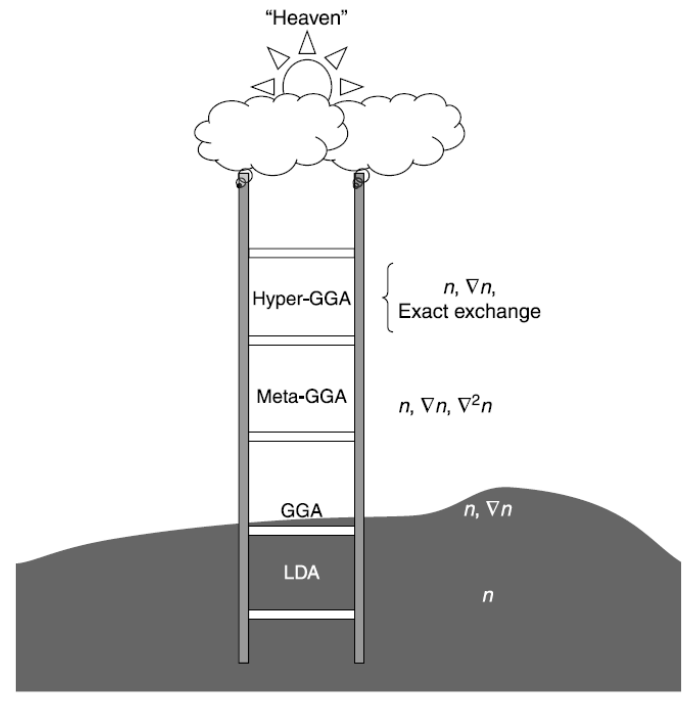
\includegraphics[height=1.7in,width=3.18in,viewport=10 5 1380 700,clip]{Figures/Jacobi-ladder.png}\\
{\small \textcolor{red}{\textrm{Jacob's ladder}}}
\end{minipage}
% \begin{itemize}%[+-| alert@+>]
%\item 交换-相关能密度泛函
}

\frame                               %
{
	\frametitle{近似能量泛函$E_{\mathrm{XC}}[\rho]$的主要问题}
\vskip 20pt
\begin{enumerate}%[+-| alert@+>]
   \setlength{\itemsep}{30pt}
 \item  密度是整体变量:电子自相互作用抵消不净%\quad\textrm{(LDA+U)}方法的校正%(\textrm{LDA+U})
 \item  电子相关:简并和近简并基态能量的表示不合理
 \item  渐近行为:处理弱相互作用体系的误差大
 \end{enumerate}
}

\frame                               %
{
	\frametitle{\textrm{Kohn-Sham}方程}
\begin{figure}[h!]
\centering
\vspace*{-0.21in}
\hspace*{-0.1in}
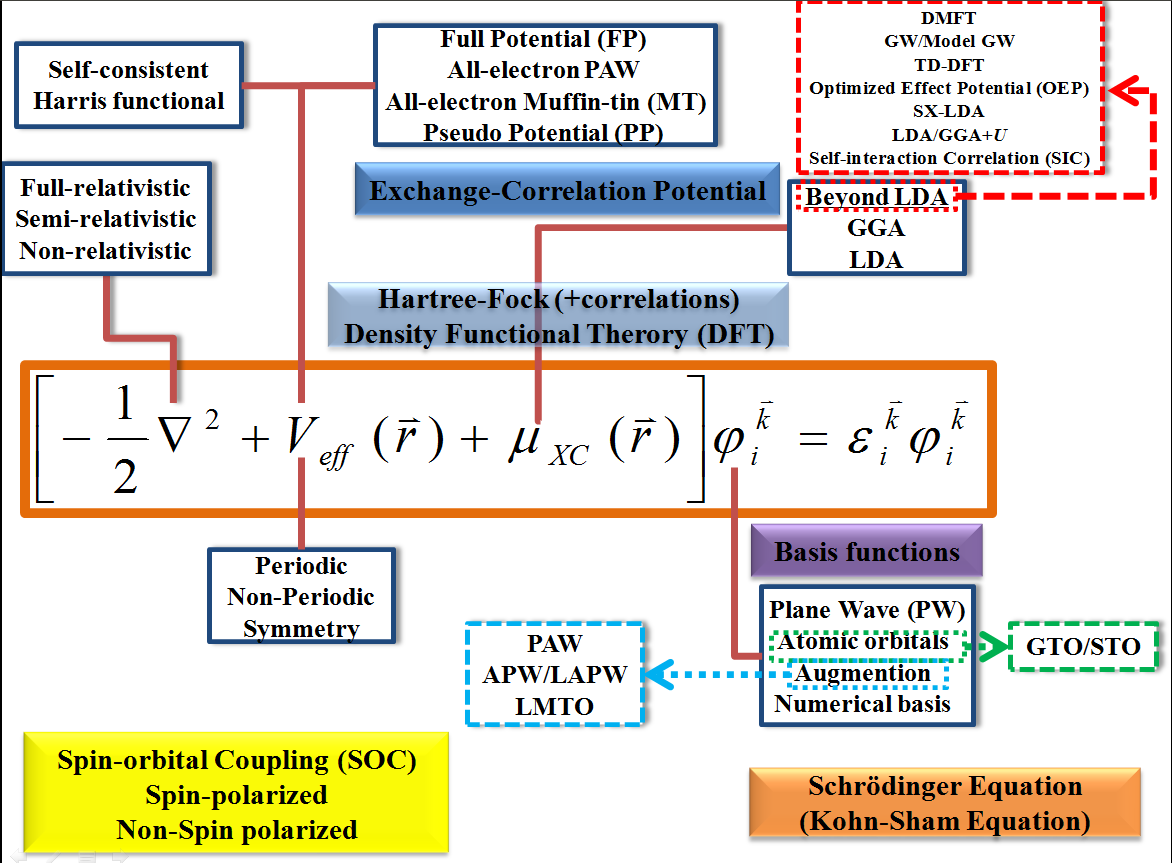
\includegraphics[height=2.7in,width=4.0in,viewport=2 5 1162 880,clip]{Figures/DFT.png}
\caption{\small \textrm{The Analysis of Kohn-Sham equation.}}%(与文献\cite{EPJB33-47_2003}图1对比)
\label{DFT}
\end{figure}
}
%\frame
%{
%\frametitle{发展统一理论框架下的材料计算程序}
%\begin{itemize}
%	\item
%\end{itemize}
%}

\appendix
%------------------------------------------------------------------------Reference----------------------------------------------------------------------------------------------
%\begin{thebibliography}{99}
%-----------------------------------------------------------------------------------------------------------------------------------------------------------------------%
%\frame
%{
%\frametitle{主要参考文献}
%{\small
%\bibitem{Singh_Book}\textrm{D. J. Singh. \textit{Plane Wave, PseudoPotential and the LAPW method} (Kluwer Academic, Boston,USA, 1994)}					%
%  \nocite{*}																				%
%}
%}
%\end{thebibliography}
\begin{thebibliography}{99}
\frame
{
\frametitle{主要参考文献}
{\small
%	\bibitem{Xu_Li_Wang}徐光宪、黎乐民、王德民, {\textit{量子化学——基本原理和从头计算法}}\;\textrm{({\textit{上、中}})}\:科学出版社, 北京, 1980
        \bibitem{PR136-B864_1964}\textrm{P. Hohenberg and W. Kohn \textit{Phys. Rev.} \textbf{136} (1964), B864}
        \bibitem{PR140-A1133_1965}\textrm{W. Kohn and L.J. Sham \textit{Phys. Rev.} \textbf{140} (1965), A1133}
	\bibitem{Parr_Yang}\textrm{R.G. Parr and W. Yang. \textit{Density-Functional Theory of Atoms and Molecules} (Oxford University Press, New York, U.S.A., 1989)}
	\bibitem{Elect_Stru}\textrm{Richard. M. Martin. \textit{Electronic Structure: Basic Theory and Practical Methods} (Cambridge University Press, Cambridge, England, 2004)}
}
\nocite*{}
}
\end{thebibliography}
%{\small
%\phantomsection\addcontentsline{toc}{section}{Bibliography}	 %直接调用\addcontentsline命令可能导致超链指向不准确,一般需要在之前调用一次\phantomsection命令加以修正	%
%\bibliography{Myref}																			%
%\bibliographystyle{mybib}																		%
%  \nocite{*}																				%
%}
%-----------------------------------------------------------------------------------------------------------------------------------------------------------------------%


%-----------------------------------------------------------Beamer下不建议使用bib,因为涉及分页--------------------------------------------------------------------------%
%{\small
%\phantomsection\addcontentsline{toc}{section}{Bibliography}	 %直接调用\addcontentsline命令可能导致超链指向不准确,一般需要在之前调用一次\phantomsection命令加以修正	%
%\bibliography{Myref}																			%
%\bibliographystyle{mybib}																		%
%  \nocite{*}																				%
%}

%------------------------------------------------------------------------------------------------------------------------------------------------------------------------------%

%-------------------------------------------------------------------------Thanks------------------------------------------------------------------------------------------------
%\section{致谢}
%\frame
%{
%\frametitle{致$\quad$谢}
%\begin{itemize}
%    \setlength{\itemsep}{20pt}
%  \item 感谢本团队高兴誉、吴泉生、宋红州等各位老师参与的讨论
%  \item 感谢莫所长、宋主任以及软件中心各位老师和同事
%  \item 感谢王崇愚先生的帮助
%\end{itemize}
%}

\logo{}									%不显示logo
\frame
{
\vskip 60 pt
%\hskip 10pt \textcolor{blue}{\Huge 感谢答辩委员会各位老师\,\textrm{!}}\\
\vskip 35 pt
\hskip 60pt \textcolor{blue}{\Huge 谢谢大家\:!}
%\vskip 15 pt
%\hskip 40pt \textcolor{blue}{\Huge \textrm{for your attention\:!}}
}

%-------------------------------------------------------------------------------------------------------------------------------------------------------------------------------

\clearpage
%\end{CJK*}
\end{document}
